\documentclass[17pt]{article}
\usepackage[top=1.6cm,bottom=1.6cm,left=1cm,right=1cm]{geometry}
%\usepackage{fontspec}
\usepackage[utf8]{inputenc}
\usepackage{hyperref}
\usepackage{enumitem}
\usepackage{changepage}
\usepackage[table]{xcolor}
\usepackage{graphicx}
\usepackage{fancyhdr}
\pagestyle{fancy}
\hypersetup{
	colorlinks=true,      
	urlcolor=magenta,
}

\title{\Huge{\textbf{Tiva Based Daughter Board for Firebird V \\ Hardware And Software Manual.}}}

\author{\textbf{ eRTS Lab IIT Bombay}}

\rhead{Manual for Tiva Based Daughter Board for Firebird V.}
\lfoot{eRTS Lab IIT Bombay}

\begin{document}
	\large
	\maketitle
	\newpage
	\section{\Huge{\textbf{Credits}}}
	\textbf{\\ \\ Version 1.0\\ \date{\today}}% Right allign
	\\
	\\
	\\
	\\
	{\large{\textbf{Documentation Author(Alphabetical Order):}
			\begin{enumerate}
			\item Ayush Gaurav, Intern eYSIP 2017
			\item Nagesh K,  Intern eYSIP 2017
	\end{enumerate}
	\textbf{Credits(Alphabetical Order):}
		\begin{enumerate}
			\item Prof Kavi Arya, CSE IIT Bombay
			\item Nex Robotics Pvt. Ltd.
			\item Piyush Manavar, Team e-Yantra
	\end{enumerate}}
	\newpage
	\section{\Huge{\textbf{Notice}}}
	{\large The contents of this manual are subject to change without notice. All efforts have been made to
	ensure the accuracy of contents in this manual. However, should any errors be detected, e-yantra welcomes your corrections. You can send us your queries / suggestions at
	\href{mailto:helpdesk@eyantra.org}{Contact Us}\\}
	\newpage
	\section{\Huge{\textbf{Index}}}%centre Allign This
	\begin{enumerate}
		\item 
	\end{enumerate}
	\newpage 
	\section{\Huge\textbf{Introduction}}
	\section{\Huge\textbf{Tiva Based Daughter Board}}
		\subsection{{\huge \textbf{Technical Specification}}}
		\subsection{}%start with the functionality
	\section{\Huge\textbf{Hardware Manual:}}
	\newpage
	\section{\Huge\textbf{Software Manual:}}
		\subsection{\huge \textbf{Code Composer Studio:}}
			{\large Code Composer Studio is an integrated development environment (IDE) that supports TI's Microcontroller and Embedded Processors portfolio. Code Composer Studio comprises a suite of tools used to develop and debug embedded applications. It includes an optimizing C/C++ compiler, source code editor, project build environment, debugger, profiler, and many other features. The intuitive IDE provides a single user interface taking you through each step of the application development flow. Familiar tools and interfaces allow users to get started faster than ever before. Code Composer Studio combines the advantages of the Eclipse software framework with advanced embedded debug capabilities from TI resulting in a compelling feature-rich development environment for embedded developers. This description is directly taken from the website of Texas Instruments and click to know more	\href{http://www.ti.com/tool/ccstudio}{about CC Studio}}}%Add an image of cc studio.
			\subsubsection{\Large\textbf{Download CC Studio:}}
			{\large At the time of writing this document Version 7 was the latest one. You can check for the latest at \href{http://processors.wiki.ti.com/index.php/Download_CCS}{Download CCS}.(do not download
				any beta versions).There will be two installer files.The web installer will require Internet access until it	completes. If the web installer version is unavailable or you can’t get it to work,
				download, unzip and run the offline version. The offline download will be much larger
				than the installed size of CCS since it includes all the possible supported hardware.}
			\subsubsection{\Large\textbf{Installing C C Studio:}}
				{After the installer has started follow the steps mentioned below:\\
				\begin{enumerate}
					\item Accept the Software License Agreement and click Next.\\
							{\centering
							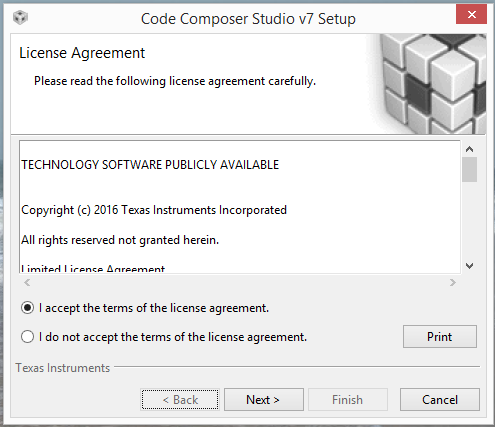
\includegraphics[width=6cm, height=6cm]{CCSInstall1}}
					\item Select the destination folder and click next.\\
							{\centering
							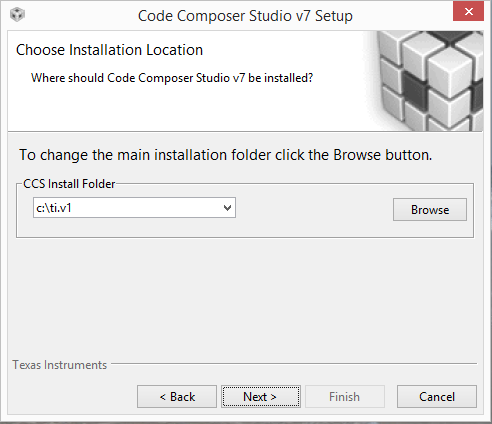
\includegraphics[width=6cm, height=6cm]{CCSInstall2}}
					\item Select the processors that your CCS installation will support. You
						must select "TM4C12X Arm Cortex M4". You can select other architectures, but the installation time and size will increase.\\{\centering
							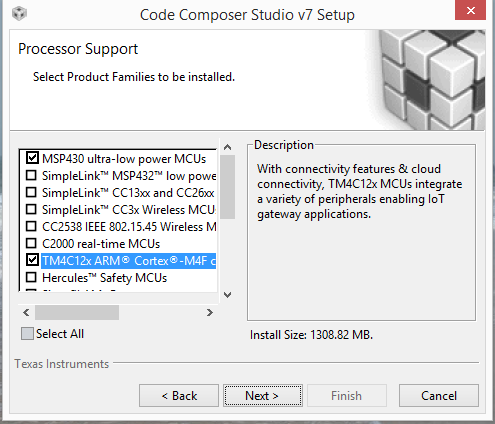
\includegraphics[width=6cm, height=6cm]{CCSInstall3}}
					\item Select debug probes and click finish \\
							{\centering
							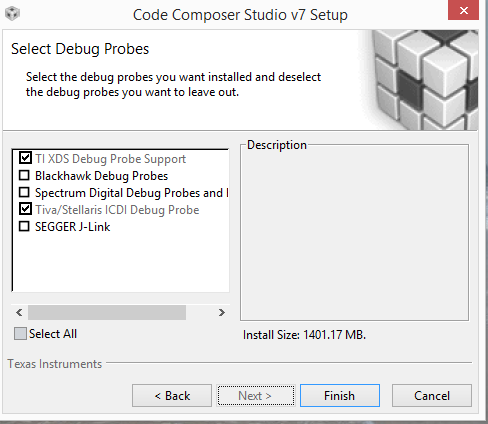
\includegraphics[width=6cm, height=6cm]{CCSInstall4}}
					\item The installer process	should take 15 - 30 minutes, depending on the speed of your connection. The offline
					installation should take 10 to 15 minutes. When the installation is complete, uncheck the
					“Launch Code Composer Studio v7” checkbox and then click Finish.There are several additional tools that require installation during the CCS install process. Click “Yes” or “OK” to proceed when these appear. \\
					\item Install TivaWare for C Series (Complete). Download and install the latest full version of TivaWare from: \href{http://www.ti.com/tool/sw-tm4c}{TivaWare}. The filename is SW-TM4C-x.x.exe . This
					workshop was built using version 1.1. Your version may be a later one. If at all possible,
					please install TivaWare into the default location.
				\end{enumerate}}
				{\large \textbf{\\You can find additional information at these websites:}\\
				Main page: www.ti.com/launchpad\\
				Tiva C Series TM4C123G LaunchPad:\\ http://www.ti.com/tool/ek-tm4c123gxl\\
				TM4C123GH6PM folder:\\ http://www.ti.com/product/tm4c123gh6pm\\
				BoosterPack webpage: www.ti.com/boosterpack\\
				LaunchPad Wiki:\\ www.ti.com/launchpadwiki\\}	\\	
				{\Large For understanding the launchpad properly and to learn more about Tiva it is strongly recommended to go through the webpage \href{http://processors.wiki.ti.com/index.php/Getting_Started_with_the_TIVA\%E2\%84\%A2_C_Series_TM4C123G_LaunchPad}{TIva Worshops} and download and read the workbook }
			\subsubsection{\huge Create a New Project}
				To create new project follow the steps mentioned:
				\begin{enumerate}
					\item Click File then New and then CCS Projects \\
						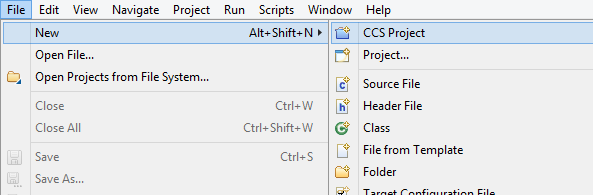
\includegraphics[width=6cm, height=2cm]{CreatingNewProject1}
					\item Select Target and connection as shown in the photo. Give a name to your project and save in a location.Click Finish. A main.c file will be open\\
						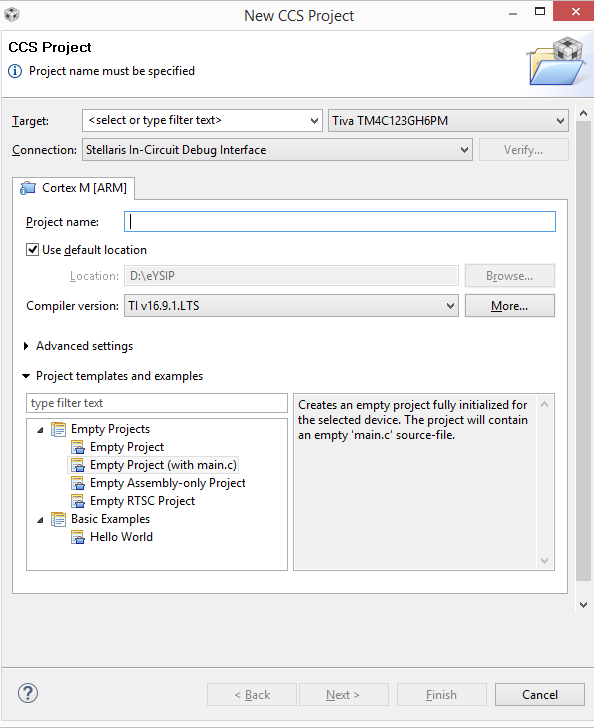
\includegraphics[width=6.5cm, height=8cm]{CreatingNewProject2}
				\end{enumerate}
			\subsubsection{\huge Add Path and Build Variables}
					{The path and build variables are used for:
					\begin{itemize}
						\item  Path variable – when you ADD (link) a file to your project, you can specify a "relative to" path. The default is PROJECT\_LOC which means that your linked resource (like a .lib	file) will be linked relative to your project directory.
						\item  Build variable – used for items such as the search path for include files associated with a library – i.e. it is used when you build your project.
				\end{itemize}
					Variables can either have a PROJECT scope (that they only work for this project) or a
					WORKSPACE scope (that they work across all projects in the workspace).
					In the next step, we need to add (link) a library file and then add a search path for include files.
					First, we’ll add these variables MANUALLY as WORKSPACE variables so that any project in your
					workspace can use the variables. Refer to the workbook by TI for adding as PROJECT}
				\subsubsection{\huge Adding a Path Variable}
					To add a path variable,:
					\begin{itemize}
						\item Right-click on your Window Tab and select Preference.\\
							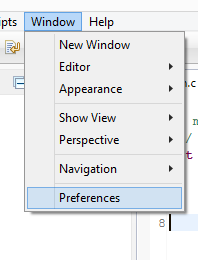
\includegraphics[width=3cm, height=4cm]{AddVariables}
						\item Expand General list  in the upper left-hand corner as shown and then expand the Resource list and click on Linked Resources:
						We want to add a New variable to specify exactly where you installed TivaWare.\\
						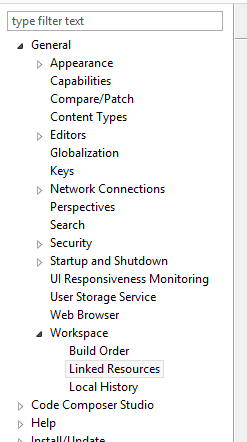
\includegraphics[height=8cm]{AddVariables2}
						\item Click New
						\item When the New Variable
						dialog appears,
						type TIVAWARE\_INSTALL
						for the name.\\
						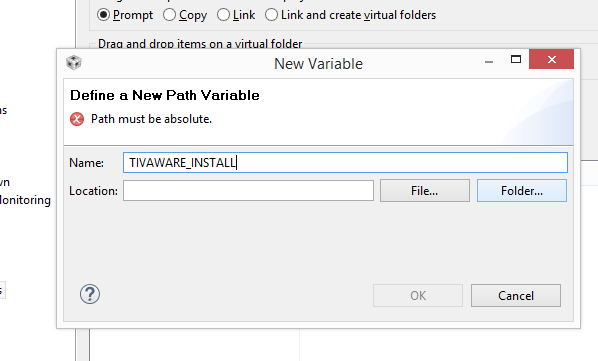
\includegraphics{AddVariables3}
						\item For the Location, click
						the Folder… button and
						navigate to your TivaWare
						installation. Click on the
						folder name and then click
						OK.\\
						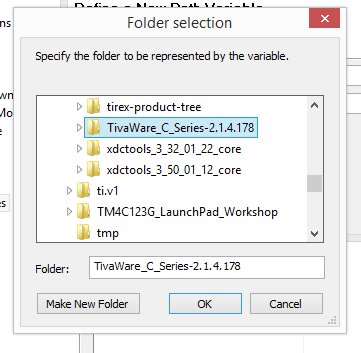
\includegraphics{AddVariables4}\\
						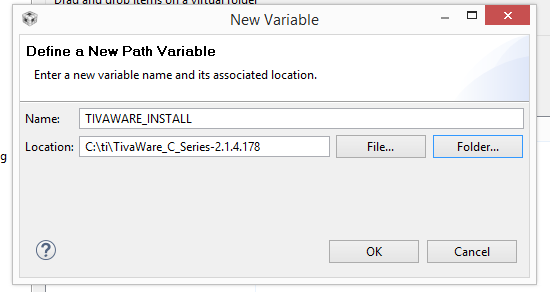
\includegraphics[width=9cm, height=8cm]{AddVariables5}
						\item Click OK. You should see your new variable listed in the Variables list.\\
						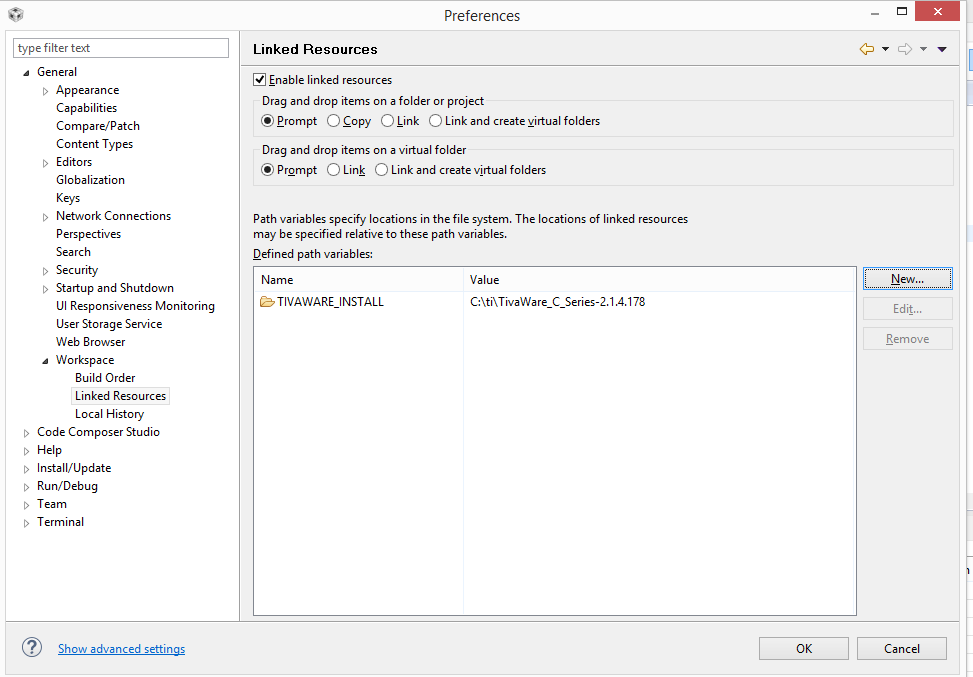
\includegraphics[width=10cm, height=8cm]{AddVariables6}
					\end{itemize}
					\subsubsection{\huge Adding a Build Variable}
					Now let’s add a build variable that we will use in the include search path for the INCLUDE files
					associated with the TivaWare driver libraries.
					\begin{itemize}
						\item Click on Code Composer Studio Build and then the Variables tab:\\
							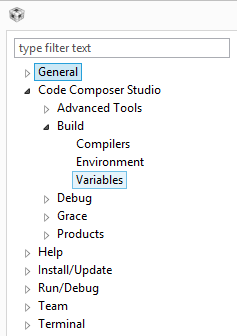
\includegraphics[width=7cm, height=8cm]{AddVariables7}\\
						\item Click the Add button. When the Define a New
						Build Variable dialog appears,
						insert TIVAWARE\_INSTALL into the Variables
						name box.\\
						\item Change the Type to Directory and
						browse to your Tivaware installation
						folder.\\
						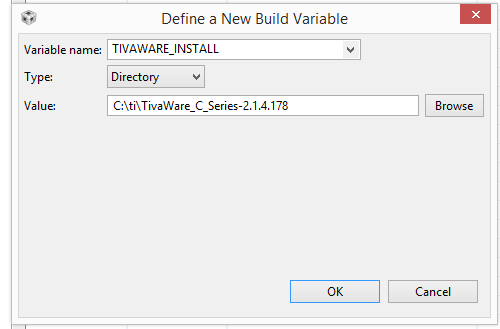
\includegraphics[width=10cm, height=8cm]{AddVariables8}
						\item  Click OK.
						\item  Click OK again to save and close
						the Build Properties window.\\
						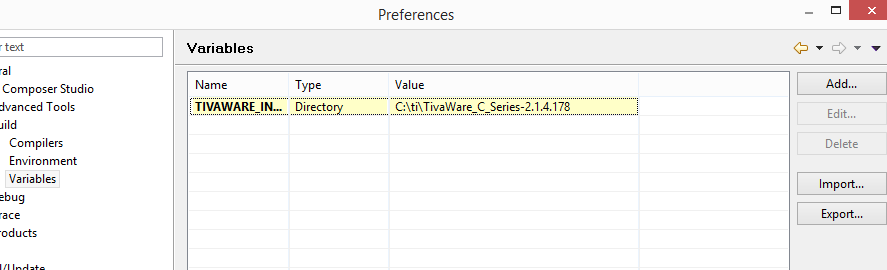
\includegraphics[width=18cm,height=12cm]{AddVariables9}
					\end{itemize}
		\subsection{Buzzer}
\end{document}